
\documentclass{elsarticle}
\usepackage{graphicx}
\usepackage{amsmath,amssymb,amsfonts,amsthm,bm}
\usepackage{hyperref}
\usepackage{booktabs,multirow}
\usepackage{lineno}
% \usepackage{cite}
\linenumbers

\bibliographystyle{elsarticle-num}
% \biboptions{longnamesfirst,angle,semicolon}

\begin{document}

\begin{frontmatter}
    \title{A Hu-Washizu variational consistent meshfree thin shell formulation with naturally accommodating essential boundary conditions}
    \author[1]{Junchao Wu\corref{cor1}}
    \ead{jcwu@hqu.edu.cn}
    \author[2]{Yangtao Xu}
    \author[1]{Bin Xu}
    \author[3]{Syed Humayun Basha}

    \affiliation[1]{organization={Key Laboratory for Intelligent Infrastructure and Monitoring of Fujian Province,
                                  College of Civil Engineering,
                                  Huaqiao University},
                    city={Xiamen},
                    state={Fujian},
                    postcode={361021},
                    country={China}}

    \affiliation[2]{organization={College of Civil Engineering,
                                  Huaqiao University},
                    city={Xiamen},
                    state={Fujian},
                    postcode={361021},
                    country={China}}

    \affiliation[3]{organization={Key Laboratory for Structural Engineering and Disaster Prevention of Fujian Province,
                                  College of Civil Engineering,
                                  Huaqiao University},
                    city={Xiamen},
                    state={Fujian},
                    postcode={361021},
                    country={China}}

    \cortext[cor1]{Corresponding author}

\begin{abstract}
A Hu-Washizu principle based variational consistent meshfree formulation with naturally enforcement of essential boundary conditions is proposed for thin shell analysis. In this approach, a mixed formulation of displacements, strains and stresses within the framework of Hu-Washizu variational principle is employed, where the displacements are discretized by meshfree shape functions, the strains and stresses are expressed as the smoothed gradients and covariant smoothed gradients which meet the first two order integration constraint and have the quasi- varational consistency. 
The numerical examples demonstrate the efficacy and efficiency of proposed method, while the RKGSI performs a comparable result in energy error with interpolation by meshfree approximations.
\end{abstract}
\begin{keyword}
Meshfree \sep Thin shell \sep Hu-Washizu variational principle \sep Reproducing kernel gradient smoothing \sep Essential boundary condition
\end{keyword}
\end{frontmatter}

\section{Introduction}


\section{Hu-Washizu's formulation of complementary energy for thin shell}\label{Kinematics}
\subsection{Kinematics for thin shell}
Consider the configuration of a shell $\bar \Omega$, as shown in Fig. \ref{}, which can be easily described by a parametric curvilinear coordinate system $\boldsymbol \xi = \{\xi^i\}_{i=1,2,3}$. The mid-surface of the shell denoted by $\Omega$ is specified by the in-plane coordinates $\boldsymbol \xi = \{\xi^\alpha\}_{\alpha=1,2}$, as the thickness direction of shell is by $\xi^3$, $-\frac{h}{2} \le \xi^3 \le \frac{h}{2}$, $h$ is the thickness of shell. In this work, Latin indices take the values from 1 to 3, and Greek indices are evaluated by 1 or 2. For the Kirchhoff hypothesis \cite{krysl1996}, the position $\boldsymbol x\in \bar \Omega$ are defined by linear functions with respect to $\xi^3$ :
\begin{equation}\label{x}
\boldsymbol x(\xi^1, \xi^2, \xi^3) = \boldsymbol r(\xi^1,\xi^2) + \xi^3 \boldsymbol a_3(\xi^1,\xi^2)
\end{equation}
in which $\boldsymbol r$ means the position on the mid-surface of shell, and the $\boldsymbol a_3$ is corresponding normal direction. For the mid-surface of shell, the in-plane covariant base vector with respect to $\xi^\alpha$ can be derived by a trivial partial differentiation to $\boldsymbol r$:
\begin{equation}
\boldsymbol a_\alpha = \frac{\partial \boldsymbol r}{\partial \xi^\alpha} = \boldsymbol r_{,\alpha}, \alpha  = 1,2
\end{equation}
for a clear expression, the subscript comma denotes the partial differentiation operation with respect to in-plane coordinates $\xi^\alpha$. And the normal vector $\boldsymbol a_3$ can be obtained by the normalized cross product of $\boldsymbol a_{\alpha}$'s as follow:
\begin{equation}
\boldsymbol a_3 = \frac{\boldsymbol a_1 \times \boldsymbol a_2}{\Vert \boldsymbol a_1 \times \boldsymbol a_2 \Vert}
\end{equation}
where $\Vert \bullet \Vert$ is the Euclidean norm operator.

With the assumption of infinitesimal deformation, the strain components respected to global contravariant base can be sated as:
\begin{equation}\label{epsilon}
\epsilon_{ij} = \frac{1}{2}(\boldsymbol x_{,i} \cdot \boldsymbol u_{,j} + \boldsymbol u_{,i} \cdot \boldsymbol x_{,j})
\end{equation}
where $\boldsymbol u$ is the displacement for shell deformation. To fulfillment with Kirchhoff hypothesis, the displacement is assumed to be the following form:
\begin{equation}\label{u}
\boldsymbol u(\xi^1,\xi^2,\xi^3) = \boldsymbol v(\xi^1,\xi^2) + \boldsymbol \theta(\xi^1,\xi^2) \xi^3
\end{equation}
in which the quadratic and higher order terms are neglected. $\boldsymbol v$, $\boldsymbol \theta$ respect the displacement and rotation in mid-surface.

Subsequently, plugging Eqs. (\ref{x}) and (\ref{u}) into Eq. (\ref{epsilon}) and neglecting quadratic terms, the strain components can be rephrased as follows:
\begin{subequations}
\begin{align}
\begin{split}
\epsilon_{\alpha\beta} &= \frac{1}{2}(\boldsymbol a_\alpha \cdot \boldsymbol v_{,\beta} + \boldsymbol v_{,\alpha}\cdot \boldsymbol a_\beta) \\ 
&+ \frac{1}{2}(\boldsymbol a_{3,\alpha} \cdot \boldsymbol v_{,\beta} + \boldsymbol v_{,\alpha}\cdot \boldsymbol a_{3,\beta} + \boldsymbol a_\alpha \cdot \boldsymbol \theta_{,\beta} + \boldsymbol \theta_{,\alpha}\cdot \boldsymbol a_\beta)\xi^3 \\
&= \varepsilon_{\alpha\beta} + \kappa_{\alpha\beta}\xi^3
\end{split} \\
\epsilon_{\alpha 3} &= \frac{1}{2}(\boldsymbol a_\alpha \cdot \boldsymbol \theta + \boldsymbol v_{,\alpha}\cdot \boldsymbol a_3) + \frac{1}{2} (\boldsymbol a_3 \cdot \boldsymbol \theta)_{,\alpha}\xi^3 \\ 
\epsilon_{33} &= \boldsymbol a_3 \cdot \boldsymbol \theta
\end{align}
\end{subequations}
where $\varepsilon_{\alpha\beta}$, $\kappa_{\alpha\beta}$ are membrane and bending strains respectively:
\begin{equation}
\varepsilon_{\alpha\beta} = \frac{1}{2}(\boldsymbol a_\alpha \cdot \boldsymbol v_{,\beta} + \boldsymbol v_{,\alpha}\cdot \boldsymbol a_\beta) 
\end{equation}
\begin{equation}\label{kappa1}
\kappa_{\alpha\beta} = \frac{1}{2}(\boldsymbol a_{3,\alpha} \cdot \boldsymbol v_{,\beta} + \boldsymbol v_{,\alpha}\cdot \boldsymbol a_{3,\beta} + \boldsymbol a_\alpha \cdot \boldsymbol \theta_{,\beta} + \boldsymbol \theta_{,\alpha}\cdot \boldsymbol a_\beta)
\end{equation}

In accordance with Kirchhoff hypothesis, the thickness of shell will not change and the deformation related with direction of $\xi^3$ will be vanished, i.e. $\epsilon_{3i}=0$. Thus, the rotation $\boldsymbol \theta$ can be rewritten as:
\begin{equation}\label{a3}
\epsilon_{3i} = 0 \Rightarrow
\left \{
\begin{split}
&\boldsymbol \theta \cdot \boldsymbol a_\alpha + \boldsymbol v_{,\alpha} \cdot \boldsymbol a_3 = 0 \\
&\boldsymbol \theta \cdot \boldsymbol a_3 = 0
\end{split}
\right .
\Rightarrow \boldsymbol \theta = - \boldsymbol v_{,\alpha} \cdot \boldsymbol a_3 \boldsymbol a^\alpha
\end{equation}
where $\boldsymbol a^\alpha$'s are the in-plane contravariant base vectors, $\boldsymbol a^\alpha \cdot \boldsymbol a_\beta = \delta^\alpha_\beta$, $\delta$ is the Kronecker delta function. Substituting Eq. (\ref{a3}) into Eq. (\ref{kappa1}) leads to:
\begin{equation}
\kappa_{\alpha\beta} = (\Gamma^\gamma_{\alpha\beta} \boldsymbol v_{,\gamma} - \boldsymbol v_{,\alpha\beta}) \cdot \boldsymbol a_3 = - \boldsymbol v_{,\alpha}\vert_\beta \cdot \boldsymbol a_3
\end{equation}
in which $\Gamma^\gamma_{\alpha\beta} = \boldsymbol a_{\alpha,\beta} \cdot \boldsymbol a^\gamma$ is namely Christoffel symbol of the second kind. And $\boldsymbol v_{,\alpha}\vert$ is the in-plane covariant derivative of $\boldsymbol v_{,\alpha}$, i.e. $\boldsymbol v_{,\alpha}\vert_\beta = \Gamma^\gamma_{\alpha\beta}\boldsymbol v_{,\gamma} - \boldsymbol v_{,\alpha\beta}$.

\subsection{Galerkin weak form for Hu-Washizu principle of complementary energy}
In this study, the Hu-Washizu variational principle of complementary energy \cite{dah-wei1985} is used herein for development of this method, the corresponding complementary functional, denoted by $\Pi_C$, is listed as follow:
\begin{equation} \label{functionalc}
\begin{split}
&\Pi_C(\varepsilon_{\alpha\beta},\kappa_{\alpha\beta},N^{\alpha\beta},M^{\alpha\beta}) \\
= &\int_\Omega \frac{h}{2}\varepsilon_{\alpha\beta} C^{\alpha\beta\gamma\eta}\varepsilon_{\gamma\eta}d\Omega 
+ \int_\Omega \frac{h^3}{24}\kappa_{\alpha\beta} C^{\alpha\beta\gamma\eta}\kappa_{\gamma\eta}d\Omega \\
+& \int_\Omega \varepsilon_{\alpha\beta} (N^{\alpha\beta} - h C^{\alpha\beta\gamma\eta} \varepsilon_{\gamma\eta}) d\Omega
+ \int_\Omega \kappa_{\alpha\beta} (M^{\alpha\beta} - \frac{h^3}{12} C^{\alpha\beta\gamma\eta} \kappa_{\gamma\eta}) d\Omega \\
-& \int_{\Gamma_v} \boldsymbol T \cdot \bar{\boldsymbol v} d\Gamma 
+ \int_{\Gamma_\theta} M_{\boldsymbol{nn}} \bar \theta_{\boldsymbol n} d\Gamma - (P \boldsymbol a_3 \cdot \bar{\boldsymbol v})_{\boldsymbol x \in C_w} \\
\end{split}
\end{equation}
where $C^{\alpha\beta\gamma\eta}$'s are the components of fourth order elasticity tensor with respect to covariant base and plane stress assumption, and it can be expressed by Young's modulus $E$, Poisson rate $\nu$ and the in-plane contravariant metric coefficients $a^{\alpha\beta}$'s, $a^{\alpha\beta} = \boldsymbol a^\alpha \cdot \boldsymbol a^\beta$, as follow: 
\begin{equation}
C^{\alpha\beta\gamma\eta} = \frac{E}{2(1+\nu)}(a^{\alpha\gamma}a^{\beta\eta} + a^{\alpha\eta}a^{\beta\gamma} + \frac{2\nu}{1-\nu} a^{\alpha\beta}a^{\gamma\eta})
\end{equation}
and $N^{\alpha\beta}$, $M^{\alpha\beta}$ are the components of membrane and bending stresses given by:
\begin{equation}
N^{\alpha\beta} = hC^{\alpha\beta\gamma\eta}\varepsilon_{\gamma\eta}, \quad
M^{\alpha\beta} = \frac{h^3}{12}C^{\alpha\beta\gamma\eta}\kappa_{\gamma\eta}
\end{equation}

Essential boundaries on the edges and corners denoted by $\Gamma_v$, $\Gamma_\theta$ and $C_v$ are naturally existed in complementary energy functional, $\bar{\boldsymbol v}$, $\bar \theta_{\boldsymbol n}$ are the corresponding prescribed displacement and normal rotation. $\boldsymbol T$, $M_{\boldsymbol{nn}}$ and $P$ can be determined by Euler-Lagrange equations of shell problem \cite{benzaken2021} as follows:
\begin{equation}
\boldsymbol T = \boldsymbol T_N + \boldsymbol T_M \; \rightarrow
\begin{cases}
\boldsymbol T_N = \boldsymbol a_\alpha N^{\alpha\beta}n_\beta \\
\boldsymbol T_M = (\boldsymbol a_3 M^{\alpha\beta}s_\alpha n_\beta)_{,\gamma} s^\gamma
+ (\boldsymbol a_3 M^{\alpha\beta})\vert_\beta n_\alpha
\end{cases}
\end{equation}
\begin{equation}
M_{\boldsymbol{nn}} = M^{\alpha\beta}n_\alpha n_\beta
\end{equation}
\begin{equation}
P = -[[M^{\alpha\beta}s_\alpha n_\beta]]
\end{equation}
where $\boldsymbol n = n^\alpha \boldsymbol a_\alpha = n_\alpha \boldsymbol a^\alpha$ and $\boldsymbol s = s^\alpha \boldsymbol a_\alpha = s_\alpha \boldsymbol a^\alpha$ are the outward normal and tangent directions on boundaries. $[[f]]$ is the jump operator defined by:
\begin{equation}
[[f]]_{\boldsymbol x = \boldsymbol x_c} = \lim_{\boldsymbol \epsilon\rightarrow \boldsymbol 0+}(f(\boldsymbol x_c + \boldsymbol \epsilon) - f(\boldsymbol x_c - \boldsymbol \epsilon)), \boldsymbol x_c \in \Gamma
\end{equation}
where $f$ is an arbitrary function on $\Gamma$.

Moreover, the natural boundary conditions should be applied by Lagrangian multiplier method with displacement $\boldsymbol v$ regarded as multiplier. Thus then the new complementary energy functional namely $\Pi$ is given by:
\begin{equation} \label{functional}
\begin{split}
&\Pi(\boldsymbol v, \varepsilon_{\alpha\beta},\kappa_{\alpha\beta},N^{\alpha\beta},M^{\alpha\beta}) \\
=&\Pi_C(\varepsilon_{\alpha\beta},\kappa_{\alpha\beta},N^{\alpha\beta},M^{\alpha\beta})
+ \int_{\Gamma_M} \theta_{\boldsymbol n} (M_{\boldsymbol{nn}} - \bar M_{\boldsymbol{nn}}) d\Gamma \\
- &\int_{\Gamma_T} \boldsymbol v \cdot (\boldsymbol T - \bar{\boldsymbol T})d\Gamma - \boldsymbol v \cdot \boldsymbol a_3 (P - \bar{P})_{\boldsymbol x \in C_P}
- \int_\Omega \boldsymbol v \cdot (\boldsymbol b - \bar{\boldsymbol b}) d\Omega 
\end{split}
\end{equation}
where $\bar{\boldsymbol T}$, $\bar M_{\boldsymbol nn}$ and $\bar P$ are the corresponding prescribed traction, bending moment and concentrated force on edges $\Gamma_T$, $\Gamma_M$ and corner $C_P$ respectively. All the boundaries meet the following geometric relationships:
\begin{equation}\label{geo}
\begin{cases}
\Gamma=\Gamma_v \cup \Gamma_T \cup \Gamma_\theta \cup \Gamma_M, \quad C = C_v \cup C_P, \\
\Gamma_v \cap \Gamma_T = \Gamma_\theta \cap \Gamma_M = C_v \cap C_P = \varnothing
\end{cases}
\end{equation}
and $\bar{\boldsymbol b}$ stands for the prescribed body force in $\Omega$, $\boldsymbol b$ also can be given based upon Euler-Lagrange equations \cite{benzaken2021} as:
\begin{equation}
\boldsymbol b = \boldsymbol b_N + \boldsymbol b_M \rightarrow
\begin{cases}
\boldsymbol b_N = (\boldsymbol a_\alpha N^{\alpha\beta})\vert_\beta \\
\boldsymbol b_M = (\boldsymbol a_3 M^{\alpha\beta})\vert_{\alpha\beta}
\end{cases}
\end{equation}

Introducing a standard variational argument to Eq. (\ref{functional}), $\delta \Pi=0$, and considering the arbitrariness of virtual variables, $\delta \boldsymbol v$, $\delta \varepsilon_{\alpha\beta}$, $\delta \kappa_{\alpha\beta}$, $N^{\alpha\beta}$, $M^{\alpha\beta}$ lead to the following weak form:
\begin{subequations}
\begin{equation}\label{w1}
- \int_\Omega h \delta \varepsilon_{\alpha\beta} C^{\alpha\beta\gamma\eta}\varepsilon_{\gamma\eta}d\Omega 
+ \int_\Omega \delta \varepsilon_{\alpha\beta} N^{\alpha\beta} d\Omega = 0
\end{equation}
\begin{equation}\label{w2}
- \int_\Omega \frac{h^3}{12} \delta \kappa_{\alpha\beta} C^{\alpha\beta\gamma\eta}\kappa_{\gamma\eta}d\Omega 
+ \int_\Omega \delta \kappa_{\alpha\beta} M^{\alpha\beta} d\Omega = 0
\end{equation}
\begin{multline}\label{w3}
\int_\Omega \delta N^{\alpha\beta} \varepsilon_{\alpha\beta} d\Omega
- \int_\Gamma \delta \boldsymbol T_N \cdot \boldsymbol v d\Gamma 
+ \int_\Omega \delta \boldsymbol b_N \cdot \boldsymbol v d\Omega \\
+ \int_{\Gamma_v} \delta \boldsymbol T_N \cdot \boldsymbol v d\Gamma 
= \int_{\Gamma_v} \delta \boldsymbol T_N \cdot \bar{\boldsymbol v} d\Gamma 
\end{multline}
\begin{multline}\label{w4}
\int_\Omega \delta M^{\alpha\beta} \kappa_{\alpha\beta} d\Omega 
- \int_\Gamma \delta M_{\boldsymbol{nn}} \theta_{\boldsymbol n}d\Gamma
+ \int_\Gamma \delta \boldsymbol T_M \cdot \boldsymbol v d\Gamma
+ (\delta P \boldsymbol a_3 \cdot \boldsymbol v)_{\boldsymbol x \in C}
+ \int_\Omega \delta \boldsymbol b_M \cdot \boldsymbol v d\Omega \\
+ \int_{\Gamma_\theta} \delta M_{\boldsymbol{nn}} \theta_{\boldsymbol n}d\Gamma
- \int_{\Gamma_v} \delta \boldsymbol T_M \cdot \boldsymbol v d\Gamma
- (\delta P \boldsymbol a_3 \cdot \boldsymbol v)_{\boldsymbol x \in C_v} \\ =
\int_{\Gamma_\theta} \delta M_{\boldsymbol{nn}} \bar{\theta}_{\boldsymbol n}d\Gamma
- \int_{\Gamma_v} \delta \boldsymbol T_M \cdot \bar{\boldsymbol v} d\Gamma
- (\delta P \boldsymbol a_3 \cdot \bar{\boldsymbol v})_{\boldsymbol x \in C_v}
\end{multline}
\begin{multline}\label{w5}
\int_{\Gamma} \delta \theta_{\boldsymbol n} M_{\boldsymbol{nn}} d\Gamma
    - \int_\Gamma \delta \boldsymbol v \cdot \boldsymbol T d\Gamma 
    - (\delta \boldsymbol v \cdot \boldsymbol a_3 P)_{\boldsymbol x \in C}
    + \int_\Omega \delta \boldsymbol v \cdot \boldsymbol b d\Omega \\
    - \int_{\Gamma_\theta} \delta \theta_{\boldsymbol n} M_{\boldsymbol{nn}} d\Gamma
    + \int_{\Gamma_v} \delta \boldsymbol v \cdot \boldsymbol T d\Gamma 
    + (\delta \boldsymbol v \cdot \boldsymbol a_3 P)_{\boldsymbol x \in C_v}
    = - \int_{\Gamma_T} \delta \boldsymbol v \cdot \bar{\boldsymbol t} d\Gamma - \int_\Omega \delta \boldsymbol v \cdot \bar{\boldsymbol b} d\Omega
\end{multline}
\end{subequations}
where the geometric relationships of Eq. (\ref{geo}) is used herein.

\section{Mixed meshfree formulation for modified Hellinger-Reissner weak form}\label{mixed}
\subsection{Reproducing kernel approximation for displacement}
This study approximates the displacement by adopting reproducing kernel approximation. As shown in Fig. \ref{fig2}, the mid-surface of the shell $\Omega$ is discretized by a set of meshfree nodes $\{\boldsymbol \xi_I\}_{I=1}^{n_p}$ in parametric configuration, where $n_p$ is the total number of meshfree nodes. The approximated displacement namely $\boldsymbol v^h$ can be expressed as:
\begin{equation}\label{approxv}
\boldsymbol v(\boldsymbol \xi) = \sum_{I=1}^{n_p} \Psi_I(\boldsymbol \xi) \boldsymbol d_I
\end{equation}
in which $\Psi_I$ and $\boldsymbol d_I$ is the shape function and nodal coefficient tensor related by node $\boldsymbol \xi_I$. According to reproducing kernel approximation \cite{liu1995}, the shape function takes the following form:
\begin{equation}
\Psi_I(\boldsymbol \xi) = \boldsymbol p^T(\boldsymbol \xi) \boldsymbol c(\boldsymbol \xi) \phi(\boldsymbol \xi_I - \boldsymbol \xi)
\end{equation}
where $\boldsymbol p$ is the basis function vector represented using the following quadratic function as:
\begin{equation}
        \boldsymbol p = \{1,\;\xi^1,\;\xi^2,\;(\xi^1)^2,\xi^1\xi^2,(\xi^2)^2\}^T
\end{equation}

The kernel function denoted by $\phi$ controls the support and smoothness of meshfree shape functions. The quintic B-spline function with square support is used herein as the kernel function:
\begin{equation}
\phi(\boldsymbol \xi_I - \boldsymbol \xi) = \phi(\hat s_1)\phi(\hat s_2), \quad \hat s_\alpha = \frac{\vert \xi^\alpha_I - \xi^\alpha\vert}{s_{\alpha I}}
\end{equation}
with
\begin{equation}
\phi(\hat s_\alpha) = \frac{1}{5!}\begin{cases}
(3-3\hat s_\alpha)^5 - 6(2-3\hat s_\alpha)^5 + 15(1-3\hat s_\alpha)^5 & \hat s_\alpha \le \frac{1}{3} \\
(3-3\hat s_\alpha)^5 - 6(2-3\hat s_\alpha)^5 & \frac{1}{3}<\hat s_\alpha \le \frac{2}{3} \\
(3-3\hat s_\alpha)^5 & \frac{2}{3}<\hat s_\alpha \le 1 \\
0 & \hat s_\alpha >1
\end{cases}
\end{equation}
and $\hat s_{\alpha I}$ means the characterized size of support for meshfree shape function $\Psi_I$.

The unknown vector $\boldsymbol c$ in shape function are determined by the fulfillment of the so-called consistency condition:
\begin{equation}
\sum_{I=1}^{n_p} \Psi_I(\boldsymbol \xi)\boldsymbol p(\boldsymbol \xi_I) = \boldsymbol p(\boldsymbol \xi)
\end{equation}
or equivalently
\begin{equation}\label{cc}
\sum_{I=1}^{n_p} \Psi_I(\boldsymbol \xi)\boldsymbol p(\boldsymbol \xi_I-\boldsymbol \xi) = \boldsymbol p(\boldsymbol 0)
\end{equation}
Substituting Eq. (\ref{approxv}) into (\ref{cc}), yields:
\begin{equation}\label{A}
\boldsymbol A(\boldsymbol \xi) \boldsymbol c(\boldsymbol \xi) = \boldsymbol p(\boldsymbol 0)\quad \Rightarrow \quad
\boldsymbol c(\boldsymbol \xi) = \boldsymbol A^{-1}(\boldsymbol \xi)\boldsymbol p(\boldsymbol 0)
\end{equation}
where $\boldsymbol A$ is the moment matrix:
\begin{equation}
\boldsymbol A(\boldsymbol \xi) = \sum_{I=1}^{n_p}\phi(\boldsymbol \xi_I - \boldsymbol \xi) \boldsymbol p(\boldsymbol \xi_I-\boldsymbol \xi)\boldsymbol p^T(\boldsymbol \xi_I - \boldsymbol \xi)
\end{equation}
Substituting Eq. (\ref{A}) back into Eq. (\ref{approxv}), the expression of meshfree shape function can be written as:
\begin{equation}
\Psi_I(\boldsymbol \xi) = \boldsymbol p^T(\boldsymbol \xi_I - \boldsymbol \xi)\boldsymbol A^{-1}(\boldsymbol \xi) \boldsymbol p(\boldsymbol 0) \phi(\boldsymbol \xi_I-\boldsymbol \xi)
\end{equation}
\subsection{Reproducing kernel gradient smoothing approximation for effective stress and strain}
In Galerkin meshfree formulation, the mid-plane of thin shell $\Omega$ is split by a set of integration cells $\Omega_C$'s, $\cup_{C=1}^{n_e}\Omega_C\approx \Omega$, as shown in Fig. \ref{fig2}. With the inspiration of reproducing kernel smoothing framework, the Cartesian and covariant derivatives of displacement, $\boldsymbol v_{,\alpha}$ and $-\boldsymbol v_{,\alpha}\vert_\beta$, in strains $\varepsilon_{\alpha\beta}$, $\kappa_{\alpha\beta}$ are approximated by $(p-1)$-th order polynomials in each integration cells. In integration cell $\Omega_C$, the approximated derivatives and strains denoted by $\boldsymbol v^h_{,\alpha}$, $\varepsilon^h_{\alpha\beta}$ and $-\boldsymbol v^h_{,\alpha}\vert_\beta$, $\kappa^h_{\alpha\beta}$ can be expressed by:
\begin{equation}\label{approxsn1}
    \boldsymbol v^h_{,\alpha}(\boldsymbol \xi) = \boldsymbol q^T(\boldsymbol \xi) \boldsymbol d_{\alpha}^\varepsilon, \quad
    \varepsilon^h_{\alpha\beta}(\boldsymbol \xi) = \boldsymbol q^T(\boldsymbol \xi) \frac{1}{2}(\boldsymbol a_\alpha \cdot \boldsymbol d_{\beta}^\varepsilon + \boldsymbol a_\beta \cdot \boldsymbol d_{\alpha}^\varepsilon)
\end{equation}
\begin{equation}\label{approxsn2}
    -\boldsymbol v^h_{,\alpha}\vert_\beta(\boldsymbol \xi) = \boldsymbol q^T(\boldsymbol \xi) \boldsymbol d_{\alpha\beta}^\kappa , \quad
    \kappa^h_{\alpha\beta}(\boldsymbol \xi) = \boldsymbol q^T(\boldsymbol \xi) \boldsymbol a_3 \cdot \boldsymbol d_{\alpha\beta}^\kappa
\end{equation}
where $\boldsymbol q$ is the linear polynomial vector and has the following form:
\begin{equation}
\boldsymbol q = \{ 1,\; \xi^1,\; \xi^2\}^T
\end{equation}
and the $\boldsymbol d^\varepsilon_{\alpha}$, $\boldsymbol d^\kappa_{\alpha\beta}$ are the corresponding coefficient vector tensors. For the conciseness, the mixed usage of tensor and vector is introduced in this study. For instance, the component of coefficient tensor vector $\boldsymbol d^\varepsilon_{\alpha I}$, $\boldsymbol d^\varepsilon_\alpha = \{\boldsymbol d^\varepsilon_{\alpha I}\}$, is a three dimensional tensor, $\dim \boldsymbol d^\varepsilon_{\alpha I} = \dim \boldsymbol v$.

\begin{figure}[!ht]
\centering
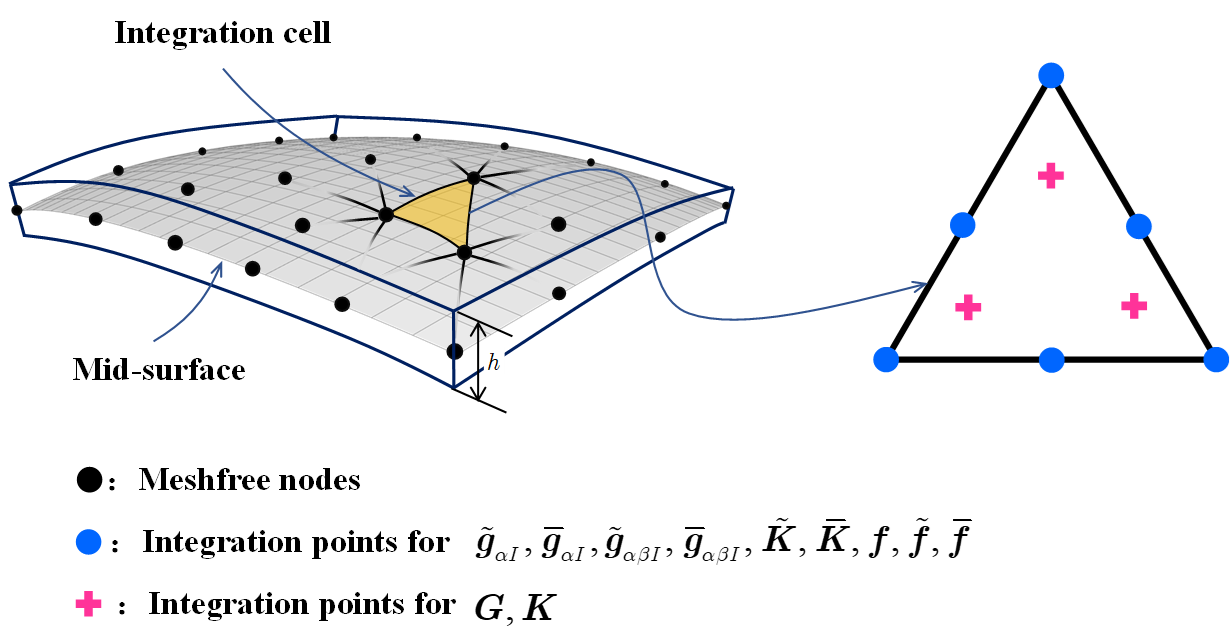
\includegraphics[width=\textwidth]{figures/2}
\caption{Integration scheme for Hu-Washizu weak form.}\label{fig2}
\end{figure}

In order to meet the integration constraint of thin shell problem, the approximated stresses $N^{\alpha\beta h}$, $M^{\alpha\beta h}$ are assumed to be a similar form with strains, yields:
\begin{equation}\label{approxse1}
N^{\alpha\beta h}(\boldsymbol \xi) = \boldsymbol q^T(\boldsymbol \xi) \boldsymbol a^\alpha \cdot \boldsymbol d^{\beta}_N,\quad
\boldsymbol a_\alpha N^{\alpha\beta h}(\boldsymbol \xi) = \boldsymbol q^T(\boldsymbol \xi) \boldsymbol d_N^\beta
\end{equation}
\begin{equation}\label{approxse2}
    M^{\alpha\beta h}(\boldsymbol \xi) = \boldsymbol q^T(\boldsymbol \xi) \boldsymbol a_3 \cdot \boldsymbol d^{\alpha\beta}_M,\quad
    \boldsymbol a_3 M^{\alpha\beta h}(\boldsymbol \xi) = \boldsymbol q^T(\boldsymbol \xi) \boldsymbol d^{\alpha\beta}_M
\end{equation}
substituting the approximations of Eqs. (\ref{approxv}), (\ref{approxsn1}), (\ref{approxsn2}), (\ref{approxse1}), (\ref{approxse2}) into Eqs. (\ref{w3}), (\ref{w4}) can express $\boldsymbol d^\varepsilon_\beta$ and $\boldsymbol d^\kappa_{\alpha\beta}$ by $\boldsymbol d$ as:
\begin{equation}\label{depsilon}
\boldsymbol d^\varepsilon_\beta = \boldsymbol G^{-1} \left (\sum_{I=1}^{n_p}(\tilde{\boldsymbol g}_{\beta I} - \bar{\boldsymbol g}_{\beta I}) \boldsymbol d_I + \hat{\boldsymbol g}_\beta \right )
\end{equation}
\begin{equation}\label{dkappa}
\boldsymbol d^\kappa_{\alpha\beta} = \boldsymbol G^{-1} \left (\sum_{I=1}^{n_p}(\tilde{\boldsymbol g}_{\alpha\beta I} - \bar{\boldsymbol g}_{\alpha\beta I})\boldsymbol d_I + \hat{\boldsymbol g}_{\alpha\beta} \right )
\end{equation}
with
\begin{equation}
\boldsymbol G = \int_{\Omega_C} \boldsymbol q^T \boldsymbol q d\Omega
\end{equation}
\begin{subequations}\label{gn}
\begin{align}
\tilde{\boldsymbol g}_{\beta I} &= \int_{\Gamma_C} \Psi_I \boldsymbol q n_\beta d\Gamma
- \int_{\Omega_C} \Psi_I \boldsymbol q_{\vert \beta} d\Omega \\
\bar{\boldsymbol g}_{\beta I} &= \int_{\Gamma_C\cap\Gamma_v} \Psi_I \boldsymbol q n_\beta d\Gamma \\
\hat{\boldsymbol g}_{\beta} &= \int_{\Gamma_C\cap\Gamma_v} \boldsymbol q n_\beta \bar{\boldsymbol v} d\Gamma 
\end{align}
\end{subequations}
\begin{subequations}\label{gm}
\begin{align}
\small
\begin{split}
\tilde{\boldsymbol g}_{\alpha\beta I} &= \int_{\Gamma_C} \Psi_{I,\gamma}n^\gamma \boldsymbol q n_\alpha n_\beta d\Gamma 
- \int_{\Gamma_C} \Psi_I(\boldsymbol q_{\vert \beta} n_\alpha + (\boldsymbol q s_\alpha n_\beta)_{,\gamma}s^\gamma) d\Gamma \\
&+ [[\Psi_I \boldsymbol q s_\alpha n_\beta]]_{\boldsymbol x\in C_C}
- \int_{\Omega_C} \Psi \boldsymbol q_{,\alpha\vert \beta} d\Omega \\
\end{split} \\
\small
\begin{split}
\bar{\boldsymbol g}_{\alpha\beta I} &= \int_{\Gamma_C\cap\Gamma_\theta} \Psi_{I,\gamma}n^\gamma \boldsymbol q n_\alpha n_\beta d\Gamma 
- \int_{\Gamma_C\cap\Gamma_v} \Psi_I(\boldsymbol q_{\vert \beta} n_\alpha + (\boldsymbol q s_\alpha n_\beta)_{,\gamma}s^\gamma) d\Gamma \\
&+ [[\Psi_I \boldsymbol q s_\alpha n_\beta]]_{\boldsymbol x\in C_C\cap C_v}
\end{split} \\
\small
\begin{split}
\hat{\boldsymbol g}_{\alpha\beta} &= \int_{\Gamma_C\cap\Gamma_\theta} \boldsymbol q n_\alpha n_\beta \boldsymbol a_3 \bar{\theta}_{\boldsymbol n} d\Gamma 
- \int_{\Gamma_C\cap\Gamma_v}(\boldsymbol q_{\vert \beta} n_\alpha + (\boldsymbol q s_\alpha n_\beta)_{,\gamma}s^\gamma)\bar{\boldsymbol v} d\Gamma \\
&+ [[\boldsymbol q s_\alpha n_\beta \bar{\boldsymbol v}]]_{\boldsymbol x\in C_C\cap C_v}
\end{split}
\end{align}
\end{subequations}
where evaluations of $\boldsymbol q_{\vert \beta}$, $\boldsymbol q_{,\alpha\vert\beta}$ are detail in \ref{derivative}. Further plugging Eqs. (\ref{depsilon}) and (\ref{dkappa}) back into Eqs. (\ref{approxsn1}) and (\ref{approxsn2}) respectively gives the final expression of $\boldsymbol v^h_{,\alpha}$, $\varepsilon^h_{\alpha\beta}$ and $-\boldsymbol v^h_{,\alpha\beta}$, $\boldsymbol \kappa^h_{\alpha\beta}$ as: \begin{subequations}
\begin{equation}
\boldsymbol v^h_{,\alpha} = \sum_{I=1}^{n_p}(
\tilde \Psi_{I,\alpha} - \bar \Psi_{I,\alpha}) \boldsymbol d_I +
\boldsymbol q^T \boldsymbol G^{-1}\hat{\boldsymbol g}_{\alpha}
\end{equation}
\begin{equation}\label{epsilonh}
\begin{split}
\varepsilon^h_{\alpha\beta} &= 
\sum_{I=1}^{n_p} \frac{1}{2}(\boldsymbol a_\alpha \tilde \Psi_{I,\beta} + \boldsymbol a_\beta \tilde \Psi_{I,\alpha}) \cdot \boldsymbol d_I 
- \sum_{I=1}^{n_p} \frac{1}{2}(\boldsymbol a_\alpha \bar \Psi_{I,\beta} + \boldsymbol a_\beta \bar \Psi_{I,\alpha}) \cdot \boldsymbol d_I \\
&+ \boldsymbol q^T \boldsymbol G^{-1} \frac{1}{2}(\boldsymbol a_\alpha \cdot \hat{\boldsymbol g}_{\beta} + \boldsymbol a_\beta \cdot \hat{\boldsymbol g}_{\alpha}) \\
&= \tilde \varepsilon^h_{\alpha\beta} - \bar \varepsilon^h_{\alpha\beta} + \hat \varepsilon^h_{\alpha\beta}
\end{split}
\end{equation}
\end{subequations}
\begin{subequations}
\begin{equation}
-\boldsymbol v^h_{,\alpha}\vert_\beta = \sum_{I=1}^{n_p} (
\tilde \Psi_{I,\alpha\beta} -
\bar \Psi_{I,\alpha\beta} ) \boldsymbol d_I +
\boldsymbol q^T \boldsymbol G^{-1}\hat{\boldsymbol g}_{\alpha\beta}
\end{equation}
\begin{equation}\label{kappah}
\begin{split}
\kappa^h_{\alpha\beta} &= \sum_{I=1}^{n_p} \tilde \Psi_{I,\alpha\beta} \boldsymbol a_3 \cdot \boldsymbol d_I
- \sum_{I=1}^{n_p} \bar \Psi_{I,\alpha\beta} \boldsymbol a_3 \cdot \boldsymbol d_I +
\boldsymbol q^T \boldsymbol G^{-1}\boldsymbol a_3 \cdot \hat{\boldsymbol g}_{\alpha\beta} \\
&= \tilde \kappa^h_{\alpha\beta} - \bar \kappa^h_{\alpha\beta} + \hat \kappa^h_{\alpha\beta}
\end{split}
\end{equation}
\end{subequations}
with
\begin{equation}\label{epsilon2}
\left \{
\begin{split}
\tilde \varepsilon^h_{\alpha\beta} &= \sum_{I=1}^{n_p} \frac{1}{2}(\boldsymbol a_\alpha \tilde \Psi_{I,\beta} + \boldsymbol a_\beta \tilde \Psi_{I,\alpha}) \cdot \boldsymbol d_I
=\sum_{I=1}^{n_p} \tilde{\boldsymbol \varepsilon}_{\alpha\beta I} \cdot \boldsymbol d_I \\
\bar \varepsilon^h_{\alpha\beta} &= \sum_{I=1}^{n_p} \frac{1}{2}(\boldsymbol a_\alpha \bar \Psi_{I,\beta} + \boldsymbol a_\beta \bar \Psi_{I,\alpha}) \cdot \boldsymbol d_I
=\sum_{I=1}^{n_p} \bar{\boldsymbol \varepsilon}_{\alpha\beta I} \cdot \boldsymbol d_I \\
\hat \varepsilon^h_{\alpha\beta} &= \boldsymbol q^T \boldsymbol G^{-1} \frac{1}{2}(\boldsymbol a_\alpha\cdot\hat{\boldsymbol g}_\beta + \boldsymbol a_\beta \cdot \hat{\boldsymbol g}_\alpha)
\end{split}
\right .
\end{equation}
\begin{equation}
\left \{
\begin{split}
&\tilde{\Psi}_{I,\alpha}(\boldsymbol \xi) = \boldsymbol q^T(\boldsymbol \xi) \boldsymbol G^{-1} \tilde{\boldsymbol g}_{\alpha I} \\
&\bar{\Psi}_{I,\alpha}(\boldsymbol \xi) = \boldsymbol q^T(\boldsymbol \xi) \boldsymbol G^{-1} \bar{\boldsymbol g}_{\alpha I} \\
&\tilde{\boldsymbol \varepsilon}_{\alpha\beta I} = \frac{1}{2}(\boldsymbol a_\alpha \tilde \Psi_{I,\beta} + \boldsymbol a_\beta \tilde \Psi_{I,\alpha}) \\
&\bar{\boldsymbol \varepsilon}_{\alpha\beta I} = \frac{1}{2}(\boldsymbol a_\alpha \bar \Psi_{I,\beta} + \boldsymbol a_\beta \bar \Psi_{I,\alpha})
\end{split}
\right .
\end{equation}
\begin{equation}\label{kappa2}
\left \{
\begin{split}
\tilde \kappa^h_{\alpha\beta} &= \sum_{I=1}^{n_p} \tilde \Psi_{I,\alpha\beta}\boldsymbol a_3 \cdot \boldsymbol d_I 
= \sum_{I = 1}^{n_p} \tilde{\boldsymbol \kappa}_{\alpha\beta I} \cdot \boldsymbol d_I\\
\bar \kappa^h_{\alpha\beta} &= \sum_{I=1}^{n_p} \bar \Psi_{I,\alpha\beta}\boldsymbol a_3 \cdot \boldsymbol d_I
= \sum_{I = 1}^{n_p} \bar{\boldsymbol \kappa}_{\alpha\beta I} \cdot \boldsymbol d_I \\
\hat \kappa^h_{\alpha\beta} &= \boldsymbol q^T \boldsymbol G^{-1} \boldsymbol a_3 \cdot \hat{\boldsymbol g}_{\alpha\beta}
\end{split}
\right .
\end{equation}
\begin{equation}
\left \{
\begin{split}
&\tilde{\Psi}_{I,\alpha\beta}(\boldsymbol \xi) = \boldsymbol q^T(\boldsymbol \xi) \boldsymbol G^{-1} \tilde{\boldsymbol g}_{\alpha\beta I} \\
&\bar{\Psi}_{I,\alpha\beta}(\boldsymbol \xi) = \boldsymbol q^T(\boldsymbol \xi) \boldsymbol G^{-1} \tilde{\boldsymbol g}_{\alpha\beta I} \\
&\tilde{\boldsymbol \kappa}_{\alpha\beta I} = \tilde \Psi_{I,\alpha\beta}\boldsymbol a_3 \\
&\bar {\boldsymbol \kappa}_{\alpha\beta I} = \bar \Psi_{I,\alpha\beta}\boldsymbol a_3 \\
\end{split}
\right .
\end{equation}

% Furthermore, taking Eqs. (\ref{approxsn1}) and (\ref{approxsn2}) into Eqs.(\ref{w1}) and (\ref{w2}) can obtain the approximated effective stresses $N^{\alpha\beta h}$, $M^{\alpha\beta h}$ and their coefficients $\boldsymbol d_N^\beta$, $\boldsymbol d_M^{\alpha\beta}$ as:
% \begin{equation}\label{d_N1}
%  \delta \boldsymbol d^\varepsilon_\alpha \cdot \boldsymbol G^{\alpha\eta}_N \cdot \boldsymbol d^\varepsilon_\eta = \delta \boldsymbol d^\varepsilon_\alpha \cdot \boldsymbol d_N^\alpha \boldsymbol G \quad\Rightarrow \quad & \boldsymbol d_N^\alpha = \boldsymbol G^{-1} \boldsymbol G_N^{\alpha\eta} \cdot \boldsymbol d^\varepsilon_\eta
% \end{equation}
% \begin{equation}\label{d_M1}
%  \delta \boldsymbol d^\kappa_{\alpha\beta} : \boldsymbol G_M^{\alpha\beta\gamma\eta} : \boldsymbol d^\kappa_{\gamma\eta} \boldsymbol G = \delta \boldsymbol d^\kappa_{\alpha\beta} \cdot \boldsymbol d_M^{\alpha\beta} \boldsymbol G \\
% \Rightarrow \; \boldsymbol d_M^{\alpha\beta} = \boldsymbol G^{-1} \boldsymbol G_{\alpha\beta}^M \cdot \boldsymbol d^\kappa_{\gamma\eta}
% \end{equation}
% with
% \begin{equation}
% \boldsymbol G^{\alpha\eta}_N = \int_{\Omega_C} \boldsymbol a_\beta hC^{\alpha\beta\gamma\eta} \boldsymbol a_\gamma \boldsymbol q \boldsymbol q^T d\Omega
% \end{equation}
% \begin{equation}
% \boldsymbol G^{\alpha\beta\gamma\eta}_M = \int_{\Omega_C} \boldsymbol a_3 \frac{h^3}{12}C^{\alpha\beta\gamma\eta}\boldsymbol a_3 \boldsymbol q\boldsymbol q^T d\Omega
% \end{equation}
%  
% Finally, taking Eqs. (\ref{d_N1}) and (\ref{d_M1}) back to Eqs. (\ref{approxse1}), (\ref{approxse2}) can express the components of stresses as follows:
% \begin{equation}\label{Nh}
% N^{\alpha\beta h} = \boldsymbol q^T \boldsymbol G^{-1}\frac{1}{2}(\boldsymbol a^\alpha \cdot \boldsymbol G^{\beta\gamma}_{N} + \boldsymbol a^\beta \cdot \boldsymbol G^{\alpha\gamma}_N) \cdot \boldsymbol d^{\varepsilon}_\gamma
% \end{equation}
% \begin{equation}\label{Mh}
% M^{\alpha\beta h} = \boldsymbol q^T \boldsymbol G^{-1} \boldsymbol a_3 \cdot \boldsymbol G^{\alpha\beta\gamma\eta}_M \cdot \boldsymbol d^\kappa_{\gamma\eta}
% \end{equation}

It has to be noted that, referring to reproducing kernel gradient smoothing framework \cite{wang2019a}, $\tilde \Psi_{I,\alpha}$, $\tilde \Psi_{I,\alpha\beta}$ are actually the first and second order smoothed gradients in curvilinear coordinates. $\tilde{\boldsymbol g}_{\alpha I}$ and $\tilde{\boldsymbol g}_{\alpha \beta I}$ are the right hand side integration constraints for first and second order gradients, then this formulation can meet the variational consistency for the $p$-th order polynomials. It should be known that, in curved model, the variational consistency for non-polynomial functions, like trigonometric functions, should be required for the polynomial solution. Even with $p$-th order variational consistency, the proposed formulation can not exactly reproduce the solution spanned by basis functions. However, the accuracy of reproducing kernel smoothed gradients is still better that traditional meshfree formulation. Numerical examples in the section below will provide better evidence to prove the accuracy of the reproducing kernel smoothed gradients.


\section{Naturally variational enforcement for essential boundary conditions}\label{boundary}
\subsection{Discrete equilibrium equations}
With the approximated effective stresses and strains, the last equation of weak form becomes:
\begin{equation}\label{w51}
- \sum_{C=1}^{n_e}(\tilde{\boldsymbol g}^T_{\alpha I} - \bar{\boldsymbol g}^T_{\alpha I}) \boldsymbol d_N^{\alpha}
- \sum_{C=1}^{n_e}(\tilde{\boldsymbol g}^T_{\alpha\beta I} - \bar{\boldsymbol g}^T_{\alpha\beta I}) \boldsymbol d_M^{\alpha\beta} = \boldsymbol f_I
\end{equation}
where $\boldsymbol f_I$'s are the components of the traditional force vector:
\begin{equation}
        \boldsymbol f_I = \int_{\Gamma_t} \Psi_I \bar{\boldsymbol t} d\Gamma - \int_{\Gamma_M} \Psi_{I,\gamma} n^\gamma \bar M_{\boldsymbol{nn}} d\Gamma + [[\Psi_I\boldsymbol a_3 \bar P]]_{\boldsymbol x\in C_P} + \int_\Omega \Psi_I \bar{\boldsymbol b} d\Omega
\end{equation}
and further substituting coefficients $\boldsymbol d_N^\alpha$, $\boldsymbol d_M^{\alpha\beta}$ into Eq. (\ref{w51}) gives the final discrete equilibrium equations: 
\begin{equation}
\begin{split}
&- \sum_{C=1}^{n_c}(\tilde{\boldsymbol g}^T_{\alpha I} - \bar{\boldsymbol g}^T_{\alpha I}) \boldsymbol d_N^{\alpha}
- \sum_{C=1}^{n_c}(\tilde{\boldsymbol g}^T_{\alpha\beta I} - \bar{\boldsymbol g}^T_{\alpha\beta I}) \boldsymbol d_M^{\alpha\beta} \\
= &\sum_{C=1}^{n_e} \sum_{J=1}^{n_p} \left (
\begin{split}
& \boldsymbol a_\alpha \tilde{\boldsymbol g}^T_{\beta I} h C^{\alpha\beta\gamma\eta} \boldsymbol a_\gamma \tilde{\boldsymbol g}_{\eta J} 
+ \tilde{\boldsymbol g}^T_{\alpha\beta I} \boldsymbol a_3 \frac{h^3}{12}C^{\alpha\beta\gamma\eta} \boldsymbol a_3 \tilde{\boldsymbol g}_{\gamma\eta} \\
- & \boldsymbol a_\alpha \bar{\boldsymbol g}^T_{\beta I} h C^{\alpha\beta\gamma\eta} \boldsymbol a_\gamma \tilde{\boldsymbol g}_{\eta J} - \boldsymbol a_\alpha \tilde{\boldsymbol g}^T_{\beta I} h C^{\alpha\beta\gamma\eta} \boldsymbol a_\gamma \bar{\boldsymbol g}_{\eta J} \\
- & \bar{\boldsymbol g}^T_{\alpha\beta I}\boldsymbol a_3 \frac{h^3}{12} C^{\alpha\beta\gamma\eta} \boldsymbol a_3 \tilde{\boldsymbol g}_{\gamma\eta J} - \tilde{\boldsymbol g}^T_{\alpha\beta I} \boldsymbol a_3 \frac{h^3}{12} C^{\alpha\beta\gamma\eta} \boldsymbol a_3 \bar{\boldsymbol g}_{\gamma\eta J} \\
+ & \boldsymbol a_\alpha \tilde{\boldsymbol g}^T_{\beta I} h C^{\alpha\beta\gamma\eta} \boldsymbol a_\gamma \hat{\boldsymbol g}_{\eta J}
- \boldsymbol a_\alpha \bar{\boldsymbol g}^T_{\beta I} h C^{\alpha\beta\gamma\eta} \boldsymbol a_\gamma \hat{\boldsymbol g}_{\eta J} \\
+ & \tilde{\boldsymbol g}^T_{\alpha\beta I}\boldsymbol a_3 \frac{h^3}{12} C^{\alpha\beta\gamma\eta} \boldsymbol a_3 \hat{\boldsymbol g}_{\gamma\eta J} - \bar{\boldsymbol g}^T_{\alpha\beta I} \boldsymbol a_3 \frac{h^3}{12} C^{\alpha\beta\gamma\eta} \boldsymbol a_3 \hat{\boldsymbol g}_{\gamma\eta J} \\
+ & \boldsymbol a_\alpha \bar{\boldsymbol g}^T_{\beta I} h C^{\alpha\beta\gamma\eta} \boldsymbol a_\gamma \bar{\boldsymbol g}_{\eta J}
+ \bar{\boldsymbol g}^T_{\alpha\beta I}\boldsymbol a_3 \frac{h^3}{12} C^{\alpha\beta\gamma\eta} \boldsymbol a_3 \bar{\boldsymbol g}_{\gamma\eta J} 
\end{split}
\right ) \\
= &\sum_{J=1}^{n_p} (\boldsymbol K_{IJ}+\tilde{\boldsymbol K}_{IJ}+\bar{\boldsymbol K}_{IJ}) \cdot \boldsymbol d_J - \tilde{\boldsymbol f}_I - \bar{\boldsymbol f}_I
\end{split}
\end{equation}
where
\begin{equation}\label{de1}
        \boldsymbol K_{IJ} = \int_\Omega \tilde{\boldsymbol \varepsilon}_{\alpha\beta I} \tilde{\boldsymbol N}^{\alpha\beta}_J d\Omega + \int_\Omega \tilde{\boldsymbol \kappa}_{\alpha\beta I} \tilde{\boldsymbol M}^{\alpha\beta}_J d\Omega
\end{equation}
\begin{subequations}\label{de2}
\begin{align}
\begin{split}
        \tilde{\boldsymbol K}_{IJ} = &- \int_{\Gamma_v} (\Psi_I \tilde{\boldsymbol t}_J + \tilde{\boldsymbol t}_I \Psi_J) d\Gamma \\
                                     &+ \int_{\Gamma_\theta} (\Psi_{I,\gamma} n^\gamma \boldsymbol a_3 \tilde M_{\boldsymbol{nn}J} + \boldsymbol a_3 \tilde M_{\boldsymbol{nn}I} \Psi_{I,\gamma}n^\gamma)d\Gamma \\
                                     & + ([[\Psi_I \boldsymbol a_3 P_J]] + [[P_I \boldsymbol a_3 \Psi_J]])_{\boldsymbol x \in C_v}
\end{split} \\
\tilde{\boldsymbol f}_I = &- \int_{\Gamma_v} \tilde{\boldsymbol t}_I \cdot \bar{\boldsymbol v} d\Gamma + \int_{\Gamma_\theta} \tilde M_{\boldsymbol{nn}} \bar{\theta}_{\boldsymbol n} d\Gamma + [[\tilde P_I\boldsymbol a_3 \cdot \bar{\boldsymbol v}]]_{\boldsymbol x \in C_v}
\end{align}
\end{subequations}
\begin{subequations}\label{de3}
\begin{align}
\bar{\boldsymbol K}_{IJ} &= - \int_{\Gamma_v} \bar{\boldsymbol t}_I \Psi_J d\Gamma 
+ \int_{\Gamma_\theta} \boldsymbol a_3\bar M_{\boldsymbol{nn}I} \Psi_{J,\gamma}n^\gamma d\Gamma + [[\bar P_I \boldsymbol a_3 \Psi_J]]_{\boldsymbol x \in C_v} \\
\bar{\boldsymbol f}_I &= - \int_{\Gamma_v} \bar{\boldsymbol t}_I \cdot \bar{\boldsymbol v} d\Gamma + \int_{\Gamma_\theta} \bar M_{\boldsymbol{nn}} \bar{\theta}_{\boldsymbol n} d\Gamma + [[\bar P_I\boldsymbol a_3 \cdot \bar{\boldsymbol v}]]_{\boldsymbol x \in C_v}
\end{align}
\end{subequations}

The detailed derivations of Eqs (\ref{de1})-(\ref{de3}) are listed in the Appendix. As shown in these equations, the Eq. (\ref{de1}) is the conventional stiffness matrix evaluated by smoothed gradients $\tilde \Psi_{I,\alpha}$, $\tilde \Psi_{I,\alpha}\vert_\beta$, and the Eqs. (\ref{de2}) and (\ref{de3}) contribute for the enforcement of essential boundary. 

\subsection{Comparison with Nitsche's method}
The Nitsche's method for enforcing essential boundary can be regarded as a combination of Lagrangian multiplier method and penalty method, in which the Lagrangian multiplier is represented by the approximated displacement. The corresponding total potential energy functional $\Pi_P$ is given by:
\begin{equation}
\begin{split}
\Pi_P(\boldsymbol v) &= \int_\Omega \frac{1}{2}\varepsilon_{\alpha\beta} N^{\alpha\beta} d\Oemga +
\int_\Omega \frac{1}{2} \kappa_{\alpha\beta}M^{\alpha\beta} d\Omega \\
                     &- \int_{\Gamma_t} \boldsymbol v \cdot \bar{\boldsymbol t} d\Gamma 
                     + \int_{\Gamma_M} \boldsymbol v_{,\gamma} n^\gamma \boldsymbol a_3 M_{\boldsymbol{nn}} d\Gamma
                     + (\boldsymbol v \cdot \boldsymbol a_3 P)_{\boldsymbol x \in C_P}
                     - \int_\Omega \boldsymbol v \cdot \bar{\boldsymbol b} d\Omega \\
                     &- \underbrace{\int_{\Gamma_v} \boldsymbol t \cdot (\boldsymbol v - \bar{\boldsymbol v}) d\Gamma
                     + \int_{\Gamma_\theta} M_{\boldsymbol{nn}}(\theta_{\boldsymbol n} - \bar \theta_{\boldsymbol n})d\Gamma
                     + (P\boldsymbol a_3 \cdot (\boldsymbol v - \bar{\boldsymbol v}))_{\boldsymbol x \in C_v}}_{\text{consistent term}} \\
                     &+ \underbrace{\frac{\alpha_v}{2} \int_{\Gamma_v} \boldsymbol v \cdot \boldsymbol v d\Gamma 
                     + \frac{\alpha_\theta}{2} \int_{\Gamma_\theta} \theta_{\boldsymbol n}^2 d\Gamma
             + \frac{\alpha_C}{2}(\boldsymbol v \cdot \boldsymbol v)_{\boldsymbol x\in C_v}}_{\text{stabilized term}}
\end{split}
\end{equation}
where the consistent term rephrased from Lagrangian multiplier method contributes to enforce the essential boundary and meet the variational consistency condition. However the consistent term can not always ensure the coercivity of stiffness, so the penalty method is introduced to be regarded as a stabilized term. With a standard variational argument, the corresponding weak form can be stated as:
\begin{equation}
\begin{split}
\delta \Pi_P(\boldsymbol v) &= \int_\Omega\delta \varepsilon_{\alpha\beta} N^{\alpha\beta} d\Oemga +
\int_\Omega \delta \kappa_{\alpha\beta}M^{\alpha\beta} d\Omega \\
                     &- \int_{\Gamma_t} \delta \boldsymbol v \cdot \bar{\boldsymbol t} d\Gamma 
                     + \int_{\Gamma_M} \delta \boldsymbol v_{,\gamma} n^\gamma \boldsymbol a_3 M_{\boldsymbol{nn}} d\Gamma
                     + (\delta \boldsymbol v \cdot \boldsymbol a_3 P)_{\boldsymbol x \in C_P}
                     - \int_\Omega \delta \boldsymbol v \cdot \bar{\boldsymbol b} d\Omega \\
                     &- \int_{\Gamma_v} \delta \boldsymbol v \cdot \boldsymbol t d\Gamma 
                     + \int_{\Gamma_\theta} \delta \theta_{\boldsymbol n} M_{\boldsymbol{nn}}d\Gamma 
                     + (\boldsymbol v \cdot \boldsymbol a_3 P)_{\boldsymbol x \in C_v}\\
                     &- \int_{\Gamma_v} \delta \boldsymbol t \cdot (\boldsymbol v - \bar{\boldsymbol v}) d\Gamma
                     + \int_{\Gamma_\theta} \delta M_{\boldsymbol{nn}}(\theta_{\boldsymbol n} - \bar \theta_{\boldsymbol n})d\Gamma
                     + (\delta P\boldsymbol a_3 \cdot (\boldsymbol v - \bar{\boldsymbol v}))_{\boldsymbol x \in C_v} \\
                     &+ \alpha_v \int_{\Gamma_v} \delta \boldsymbol v \cdot \boldsymbol v d\Gamma 
                     + \alpha_\theta \int_{\Gamma_\theta} \delta \theta_{\boldsymbol n}\theta_{\boldsymbol n} d\Gamma
                     + \alpha_C(\delta \boldsymbol v \cdot \boldsymbol v)_{\boldsymbol x\in C_v} \\
                     &= 0
\end{split}
\end{equation}
in which $\alpha_v$, $\alpha_\theta$ and $\alpha_C$ are experimental artificial parameters. Further invoking the conventional reproducing kernel approximation of Eq. (\ref{approxv}) leads to the following discrete equilibrium equations:
\begin{equation}
\sum_{J=1}^{n_p}(\boldsymbol K_{IJ} + \boldsymbol K^c_{IJ} + \boldsymbol K^s_{IJ}) \boldsymbol d_J = \boldsymbol f_I + \boldsymbol f^c + \boldsymbol f^s
\end{equation}
where the stiffness $\boldsymbol K_{IJ}$ is identical with Eq. (\ref{de1}). $\boldsymbol K^c_{IJ}$ and $\boldsymbol K^s_{IJ}$ are the stiffness matrix for consistent and stabilized terms respectively, and have the following forms:
\begin{subequations}
\begin{equation}
\begin{split}
        \boldsymbol K^c_{IJ} &= -\int_{\Gamma_v} \left ((\boldsymbol {\mathcal T}^\alpha \Psi_{I,\alpha} + \boldsymbol{\mathcal V}^{\alpha\beta} \Psi_{I,\alpha}\vert_\beta) \Psi_J + \Psi_I (\boldsymbol {\mathcal T}^\alpha \Psi_{J,\alpha} + \boldsymbol{\mathcal V}^{\alpha\beta}\Psi_{J,\alpha}\vert_\beta)\right ) d\Gamma \\
                             &+ \int_{\Gamma_M} (\mathcal M^{\alpha\beta} \Psi_{I,\alpha}\vert_\beta \boldsymbol a_3 \Psi_{J,\gamma}n^\gamma + \Psi_{I,\gamma}n^\gamma \boldsymbol a_3 \mathcal M^{\alpha\beta} \Psi_{I,\alpha}\vert_\beta) d\Gamma
\end{split}
\end{equation}
\end{subequations}


\section{Numerical examples}
In this section, several examples are carried out to verify proposed method, which employs the consistent reproducing kernel gradient smoothing integration scheme (RKGSI) and the non-consistent Gauss integration scheme (GI) with penalty method, Nitsche's method and the proposed Hu-Washizu formulation (HW) to enforce the essential boundary conditions. A normalized support size of 2.5 is used for all methods to ensure the requirement of quadratic base meshfree approximation. To eliminate the influence of integration, the Gauss integration scheme use 6 Gauss points for domain integration and 3 points for boundary integration, and such that the number of integration points are identical between Gauss scheme and RKGSI scheme. The error estimates of displacement namely $L_2$-Error and energy namely $H_e$-Error is used here:
\begin{equation}
\begin{split}
L_2\text{-Error} &= \frac{\sqrt{\int_\Omega(\boldsymbol v - \boldsymbol v^h) \cdot (\boldsymbol v - \boldsymbol v^h)d\Omega}}{\sqrt{\boldsymbol v \cdot \boldsymbol v}} \\
H_e\text{-Error} &= \frac{\sqrt{\int_\Omega \left ((\varepsilon_{\alpha\beta} - \varepsilon_{\alpha\beta}^h)(N^{\alpha\beta} - N^{\alpha\beta h}) + \int_\Omega(\kappa_{\alpha\beta}-\kappa_{\alpha\beta}^h)(M^{\alpha\beta}-M^{\alpha\beta h}) \right )d\Omega}}{\sqrt{\int_\Omega(\varepsilon_{\alpha\beta}N^{\alpha\beta} + \kappa_{\alpha\beta}M^{\alpha\beta})d\Omega}}
\end{split}
\end{equation}

\subsection{Patch tests}
The linear and quadratic patch tests for flat and curved thin shell are firstly study to verify the variational consistency of the proposed method. As shown in Fig. \ref{ptf1}, the flat and curved model is depicted by an identical parametric domain $\Omega = (0,1)\otimes(0,1)$, where the cylindrical coordinate system with radius $R=1$ is employed to describe the curved model, and the whole domain $\Omega$ is discretized by $165$ meshfree nodes. All the boundaries are enforced as essential boundary conditions with the following manufactured exact solution:
\begin{equation}
\boldsymbol v = \begin{Bmatrix}
(\xi^1+2\xi^2)^n \\ (3\xi^1+4\xi^2)^n \\ (5\xi^1+6\xi^2)^n
\end{Bmatrix},\quad
n = \begin{cases}
1 & \text{Linear patch test} \\
2 & \text{Quadratic patch test}
\end{cases}
\end{equation}

\begin{figure}[h!]
    \centering
    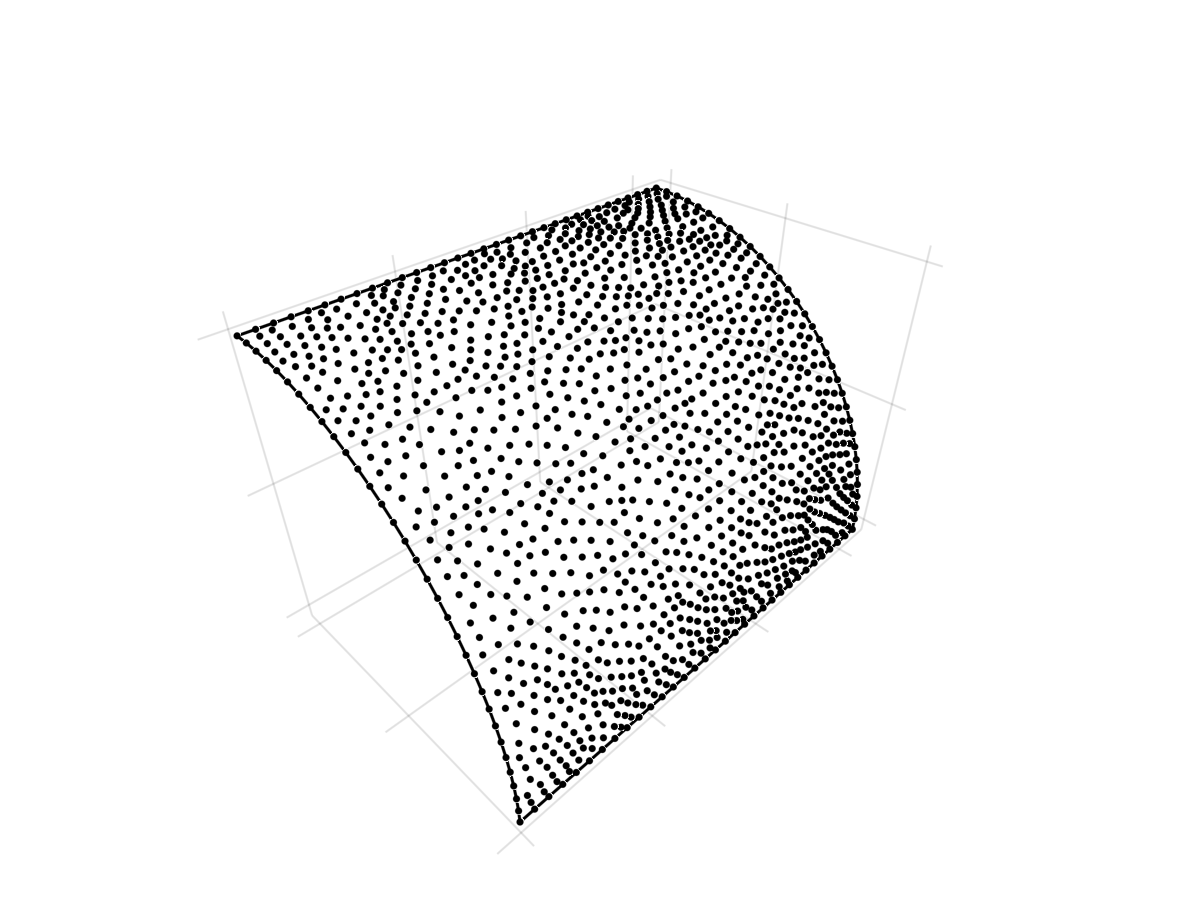
\includegraphics[width=\textwidth]{figures/patchtest_msh}
    \caption{Meshfree discretization for patch test}\label{ptf1}
\end{figure}

Table \ref{ptt1} lists the $L_2$- and $H_e$-Error results of patch test with flat model, where the RKGSI with variational consistent essential boundary enforcement, i.e. RKGSI-Nitsche and RKGSI-HW, can pass the linear and quadratic path test. Due to the loss of variational consistency condition, even with Nitsche's method, Gauss meshfree formulations show noticeable errors. Table \ref{ptt2} shows the results for curved model, which indicated that all the mehtods cannot pass the patch test, which mainly because the proposed smoothed gradient of Eqs. (\ref{approxse1}), (\ref{approxse2}) is unable to exactly reproduce the non-polynomial membrane and bending stress. However, the RKGSI-HW and RKGSI-Nitsche also performance better accuracy than other methods due to the fulfillment of first two order variational consistency. Meanwhile, the bending moment contours of $M^{12}$ are listed in Fig. \ref{ptf2}, which further verify that the proposed method obtain a satisfactory result comparing with exact solution, the conventional Gauss meshree formulations show observable errors.

\begin{table}[h!]
\centering
\caption{Results of patch test for flat model}\label{ptt1}
\begin{tabular}{lcccc}
\toprule
 & \multicolumn{2}{c}{Linear patch test} & \multicolumn{2}{c}{Quadratic patch test} \\ \cline{2-5}
 & $L_2$-Error & $H_e$-Error & $L_2$-Error & $H_e$-Error \\
    \midrule
    GI-Penalty & $4.45E-4$ & $1.35E-2$ & $2.01E-3$ & $1.63E-2$ \\
    GI-Nitsche & $4.51E-4$ & $1.42E-2$ & $1.22E-3$ & $1.68E-2$ \\
    RKGSI-Penalty & $3.64E-9$ & $6.77E-8$ & $4.54E-9$ & $6.57E-8$ \\
    RKGSI-Nitsche & $3.31E-12$ & $1.34E-11$ & $5.98E-12$ & $1.21E-11$ \\
    RKGSI-HR & $6.67E-13$ & $1.50E-11$ & $1.07E-12$ & $1.26E-11$ \\
    \bottomrule
\end{tabular}
\end{table}

\begin{table}[h!]
\centering
\caption{Results of patch test for curved model.}\label{ptt2}
\begin{tabular}{lcccc}
\toprule
 & \multicolumn{2}{c}{Linear patch test} & \multicolumn{2}{c}{Quadratic patch test} \\ \cline{2-5}
 & $L_2$-Error & $H_e$-Error & $L_2$-Error & $H_e$-Error \\
    \midrule
    GI-Penalty & $3.79E-4$ & $1.30E-2$ & $1.74E-3$ & $1.37E-2$ \\
    GI-Nitsche & $4.04E-4$ & $1.42E-2$ & $1.15E-3$ & $1.49E-2$ \\
    RKGSI-Penalty & $1.47E-4$ & $5.39E-3$ & $2.26E-4$ & $2.09E-3$ \\
    RKGSI-Nitsche & $2.41E-6$ & $7.37E-5$ & $2.47E-6$ & $2.89E-5$ \\
    RKGSI-HR & $4.28E-6$ & $1.30E-4$ & $9.69E-6$ & $2.41E-4$ \\
    \bottomrule
\end{tabular}
\end{table}

\begin{figure}[h!]
\centering
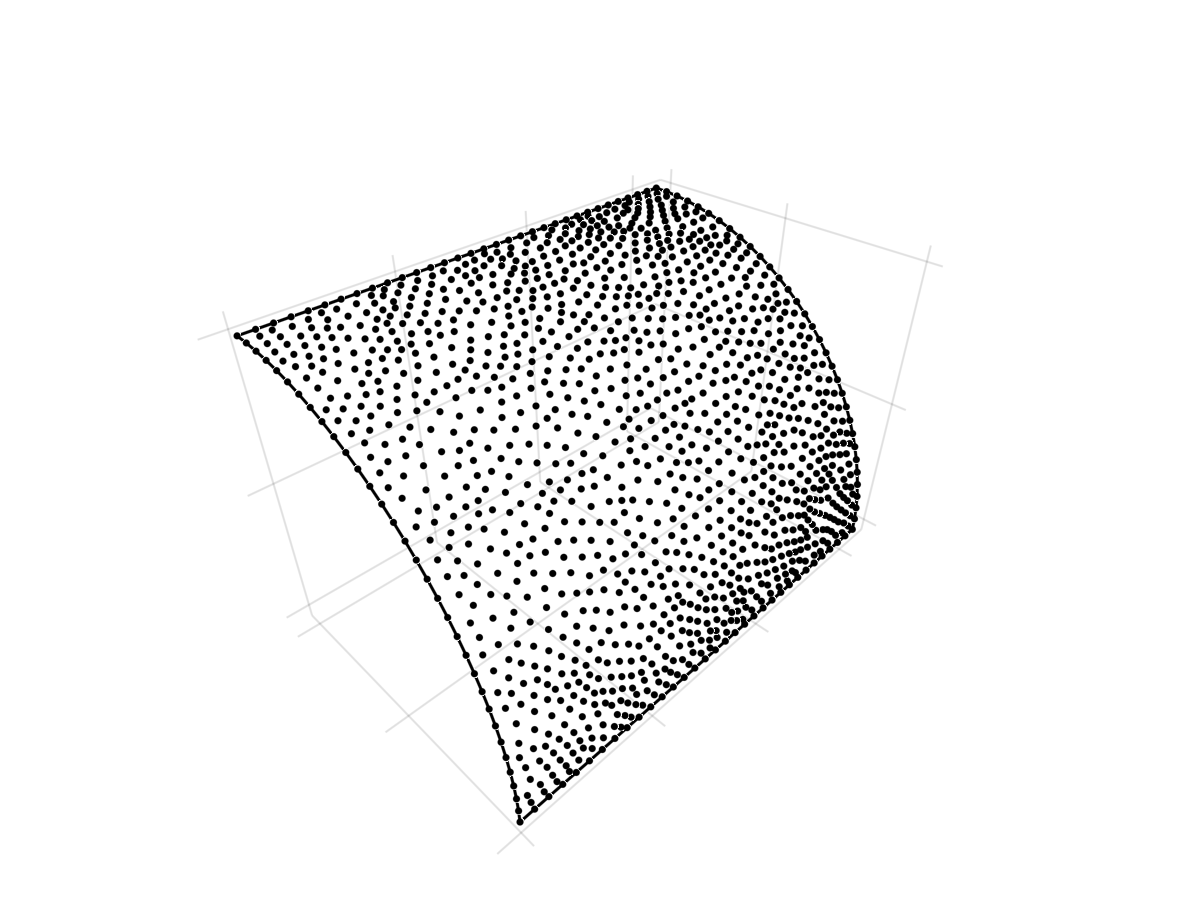
\includegraphics[width=\textwidth]{figures/patchtest_msh}
\caption{Contour plots of $M^{12}$ for curved shell patch test.}\label{ptf2}
\end{figure}

\subsection{Scordelis-Lo roof}
This example consider the classical Scordelis-Lo roof problem, as shown in Fig., the cylindrical roof has the radius $R=25$, length $L=50$, thickness $h=0.25$, Young's modulus $E=4.32\times 10^8$ and Poisson rate $\nu=0.0$. An uniform body force of $b_z = -90$ are enforced in whole roof and the curved edges are enforced by $v_x=v_z=0$, and the straight edges are free.

Due to the symmetry, only a quadrant of the model is considered for meshfree analysis, which is discretized by the $5\times 8$, $11\times 16$, $17\times 24$ and $23\times32$ meshfree nodes.

\begin{figure}[h!]
\centering
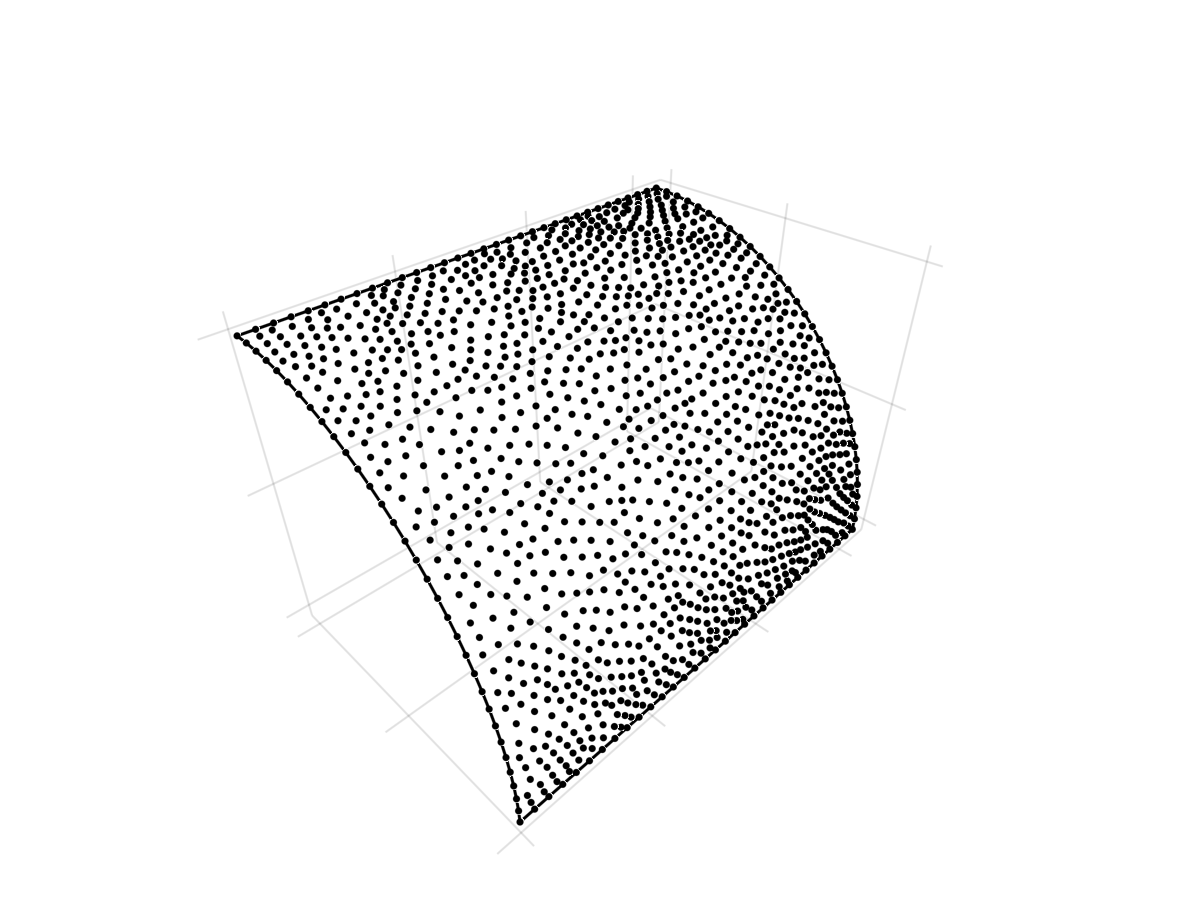
\includegraphics[width=\textwidth]{figures/patchtest_msh}
\caption{Description of Scordelis-Lo roof problem.}\label{ptf2}
\end{figure}

\section{Conclusion}\label{conclusion}
In this study, an efficient and quasi-consistent meshfree thin shell formulation was presented to naturally enforce the essential boundary conditions.  Mixed formulation with the Hu-Washizu principle weak form is adopted, where the traditional meshfree shape functions discretized the displacement, and the strains and stresses were expressed by the reproducing kernel smoothed gradients and the covariant smoothed gradients, respectively. The smoothed gradient naturally embedded the first second-order integration constraints and has a quasi variational consistency for the curved models in each integration cell. Owing to the Hu-Washizu variational principle, the essential boundary condition enforcement has a similar form with the conventional Nitsche’s method; both have consistent and stabilized terms. The costly high order derivatives in the Nitsche’s consistent term have been replaced by the smoothed gradients, which improved the computational speed due to the reproducing kernel gradient smoothing framework. Furthermore, the stabilized term naturally existed in the Hu-Washizu weak form, and the artificial parameter needed in Nitsche’s stabilized term has vanished, which can automatically maintain the coercivity for the stiffness matrix. Based on general reproducing kernel gradient smoothing framework, the proposed methodology can be trivially extended to high order basis meshfree formulation. The numerical results demonstrated that the proposed Hu-Washizu quasi-consistent meshfree thin shell formulation showed excellent accuracy, efficiency, and stability.


\section*{Acknowledgment}
The support of this work by the National Natural Science Foundation of China (12102138, 52350410467) and the Natural Science Foundation of Fujian Province of China (2023J01108, 2022J05056) is gratefully acknowledged.
\appendix
\section{Covariant derivatives}\label{appderivative}
This Appendix lists the covariant derivatives needed for the development of the proposed method. For an arbitrary first order tensor $\boldsymbol v$ presented by in-plane covariant or contravariant bases as: 
\begin{equation}
\boldsymbol v = v_{\alpha}\boldsymbol a^\alpha + v_{3} \boldsymbol a_3 = v^{\alpha}\boldsymbol a_\alpha + v^3 \boldsymbol a_3
\end{equation}
the partial derivatives of tensor $\boldsymbol v$ with respect to coordinate $\xi^\alpha$, $\boldsymbol v_{,\alpha}$, can be evaluated by:
\begin{equation}
\begin{split}
\boldsymbol v_{,\alpha} &= 
v_{\beta,\alpha} \boldsymbol a^\beta + v_{\beta}\boldsymbol a^\beta_{,\alpha} + v_{3,\alpha}\boldsymbol a_3 + v_3 \boldsymbol a_{3,\alpha} \\
&= v_{\beta,\alpha} \boldsymbol a^\beta - \Gamma^\beta_{\alpha\gamma}v_\beta \boldsymbol a^\gamma + v_{3,\alpha} \boldsymbol a_3 - v_3 b_{\alpha\beta} \boldsymbol a^\beta \\
&= v_{\beta,\alpha} \boldsymbol a^\beta - \Gamma^\gamma_{\alpha\beta}v_\gamma \boldsymbol a^\beta + v_{3,\alpha} \boldsymbol a_3 - v_3 b_{\alpha\beta} \boldsymbol a^\beta \\
&= v_{\beta}\vert_\alpha \boldsymbol a^\beta + v_{3,\alpha} \boldsymbol a_3 - v_3 b_{\alpha\beta} \boldsymbol a^\beta \\
\end{split}
\end{equation}
where $\Gamma^\gamma_{\alpha\beta} = \boldsymbol a_{\alpha,\beta}\cdot \boldsymbol a^\gamma$ denotes the Christoffel symbol of the second kind, $b_{\alpha\beta} = \boldsymbol a_{\alpha,\beta}\cdot\boldsymbol a_3=-\boldsymbol a_{\alpha}\cdot\boldsymbol a_{3,\beta}$ stands for the curvature tensor. $v_\alpha\vert_\beta$ can be regarded as the in-plane covariant derivative of the vector $v_\alpha$:
\begin{equation}
v_{\alpha}\vert_\beta = v_{\alpha,\beta} - \Gamma^\gamma_{\alpha\beta} v_\gamma
\end{equation}

Following the same path, the in-plane covariant derivative of $v^\alpha$ is given by:
\begin{equation}
v^\alpha\vert_\beta = v^\alpha_{,\beta} + \Gamma^\alpha_{\beta\gamma} v^\gamma
\end{equation}


\section{Derivations for stiffness metrics and force vectors}\label{derivations}
This Appendix details the derivations of stiffness matrices and force vectors in Eqs. (\ref{de1})-(\ref{de3}), where the relationships of Eqs. (\ref{gn}), (\ref{gm}), (\ref{epsilon2}) and (\ref{kappa2}) are used herein. Firstly, the membrane strain terms are considered as follows:
\begin{equation}
\begin{split}
&\sum_{C=1}^{n_e}\int_{\Omega_C} \delta \tilde \varepsilon_{\alpha\beta}^h hC^{\alpha\beta\gamma\eta}\bar \varepsilon^h_{\gamma\eta} d\Omega \\
        =&\sum_{C=1}^{n_e}\sum_{I,J=1}^{n_p}\delta \boldsymbol d_I \cdot \underbrace{\int_{\Omega_C} \tilde{\boldsymbol \varepsilon}_{\alpha\beta I} hC^{\alpha\beta\gamma\eta} \boldsymbol a_\gamma \boldsymbol q^T d\Omega}_{\tilde{\boldsymbol g}^{\eta T}_I} \boldsymbol G^{-1} \bar{\boldsymbol g}_{\eta J} \cdot \boldsymbol d_J \\
        =&\sum_{C=1}^{n_e}\sum_{I,J=1}^{n_p}\delta \boldsymbol d_I \cdot \int_{\Gamma_C\cap\Gamma_v} \Psi_J \underbrace{\boldsymbol q^T \boldsymbol G^{-1}\tilde{\boldsymbol g}^\alpha_I
        n_\alpha}_{\tilde{\boldsymbol T}_{NI}} d\Gamma
       \cdot \boldsymbol d_J \\
        =&\sum_{I,J=1}^{n_p}\delta \boldsymbol d_I \cdot \int_{\Gamma_v} \tilde{\boldsymbol T}_{NI}\Psi_J d\Gamma
       \cdot \boldsymbol d_J \\
\end{split}
\end{equation}
with
\begin{equation}
        \tilde{\boldsymbol g}^\alpha_I = \boldsymbol q \boldsymbol a_\beta hC^{\alpha\beta\gamma\eta} \tilde{\boldsymbol \varepsilon}_{\alpha\beta I}
\end{equation}
\begin{equation}
        \tilde{\boldsymbol T}_{NI} = \boldsymbol q^T \boldsymbol G^{-1} \tilde{\boldsymbol g}_I^\alpha n_\alpha
\end{equation}

Following this path, the bending strain terms can be reorganized by:
\begin{equation}
\begin{split}
&\sum_{C=1}^{n_e}\int_{\Omega_C} \delta \tilde \kappa_{\alpha\beta}^h \frac{h^3}{12}C^{\alpha\beta\gamma\eta}\bar \kappa^h_{\gamma\eta} d\Omega \\
        =&\sum_{C=1}^{n_e}\sum_{I,J=1}^{n_p}\delta \boldsymbol d_I \cdot \underbrace{\int_{\Omega_C} \tilde{\boldsymbol \kappa}_{\alpha\beta I} \frac{h^3}{12}C^{\alpha\beta\gamma\eta} \boldsymbol a_3 \boldsymbol q^T d\Omega}_{\tilde{\boldsymbol g}^{\gamma\eta T}_I} \boldsymbol G^{-1} \bar{\boldsymbol g}_{\gamma\eta J} \cdot \boldsymbol d_J \\
        =&\sum_{C=1}^{n_e}\sum_{I,J=1}^{n_p}\delta \boldsymbol d_I \cdot \left (
        \begin{split}
                &\int_{\Gamma_C\cap\Gamma_\theta} \underbrace{\boldsymbol q^T \boldsymbol G^{-1}\tilde{\boldsymbol g}^{\alpha\beta}_I n_\alpha n_\beta}_{\tilde{\boldsymbol M}_{\boldsymbol{nn} I}} n^\gamma\Psi_{J,\gamma} d\Gamma \\
                - &\int_{\Gamma_C\cap\Gamma_v} (\underbrace{\boldsymbol q^T_{\vert \beta} \boldsymbol G^{-1}\tilde{\boldsymbol g}^{\alpha\beta}_I n_\alpha + (\boldsymbol q^T \boldsymbol G^{-1}\tilde{\boldsymbol g}^{\alpha\beta}_I s_\alpha n_\beta)_{,\gamma}s^\gamma}_{\tilde{\boldsymbol T}_{M I}}) \Psi_J d\Gamma \\
                + &[[\underbrace{\boldsymbol q^T \boldsymbol G^{-1}\tilde{\boldsymbol g}^{\alpha\beta}_I s_\alpha n_\beta}_{\tilde{\boldsymbol P}_I \boldsymbol a_3} \Psi_J ]]_{\boldsymbol x\in C_C\cap C_v}
        \end{split}
       \right ) \cdot \boldsymbol d_J \\
       =&\sum_{I,J=1}^{n_p}\delta \boldsymbol d_I \cdot (
       \int_{\Gamma_\theta} \tilde{\boldsymbol M}_{\boldsymbol{nn} I} n^\gamma\Psi_{J,\gamma} d\Gamma
        - \int_{\Gamma_v} \tilde{\boldsymbol T}_{M I} \Psi_J d\Gamma
        + [[\tilde{\boldsymbol P}_I \Psi_J ]]_{\boldsymbol x\in C_v})
\end{split}
\end{equation}
with
\begin{equation}
\tilde{\boldsymbol g}^{\alpha\beta}_I = \int_{\Omega_C} \boldsymbol q \frac{h^3}{12}C^{\alpha\beta\gamma\eta} \boldsymbol a_3 \tilde{\boldsymbol \kappa}_{\alpha\beta I}d\Omega
\end{equation}
\begin{equation}
\left \{
\begin{split}
&\tilde{\boldsymbol M}_{\boldsymbol{nn} I} = \boldsymbol q^T \boldsymbol G^{-1}\tilde{\boldsymbol g}^{\alpha\beta}_I n_\alpha n_\beta \\
&\tilde{\boldsymbol T}_{M I} = \boldsymbol q^T_{\vert \beta} \boldsymbol G^{-1}\tilde{\boldsymbol g}^{\alpha\beta}_I n_\alpha + (\boldsymbol q^T \boldsymbol G^{-1}\tilde{\boldsymbol g}^{\alpha\beta}_I s_\alpha n_\beta)_{,\gamma}s^\gamma \\
&\tilde{\boldsymbol P}_I = \boldsymbol q^T \boldsymbol G^{-1}\tilde{\boldsymbol g}^{\alpha\beta}_I s_\alpha n_\beta \cdot \boldsymbol a_3
\end{split}
\right .
\end{equation}

\bibliography{references}
\end{document}
